\documentclass[tikz,border=10pt]{standalone}
\begin{document}
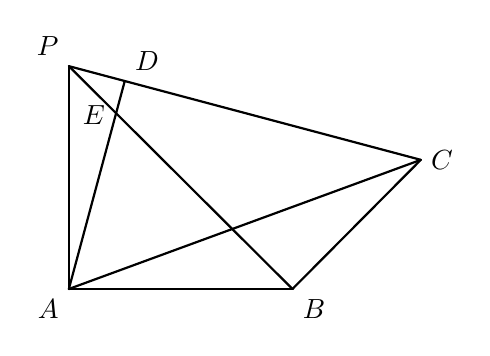
\begin{tikzpicture}[line cap=round, line join=round, thick]
\coordinate (P) at (0.68,-0.66);
\coordinate (D) at (1.39,-0.85);
\coordinate (E) at (1.27,-1.28);
\coordinate (A) at (0.68,-3.49);
\coordinate (B) at (3.52,-3.49);
\coordinate (C) at (5.15,-1.85);

\draw (P) -- (A);
\draw (A) -- (B);
\draw (B) -- (C);
\draw (P) -- (C);
\draw (P) -- (B);
\draw (A) -- (C);
\draw (A) -- (D);

\node[above left] at (P) {$P$};
\node[above right] at (D) {$D$};
\node[left] at (E) {$E$};
\node[below left] at (A) {$A$};
\node[below right] at (B) {$B$};
\node[right] at (C) {$C$};
\end{tikzpicture}
\end{document}
